\documentclass[tikz]{standalone}
\begin{document}
	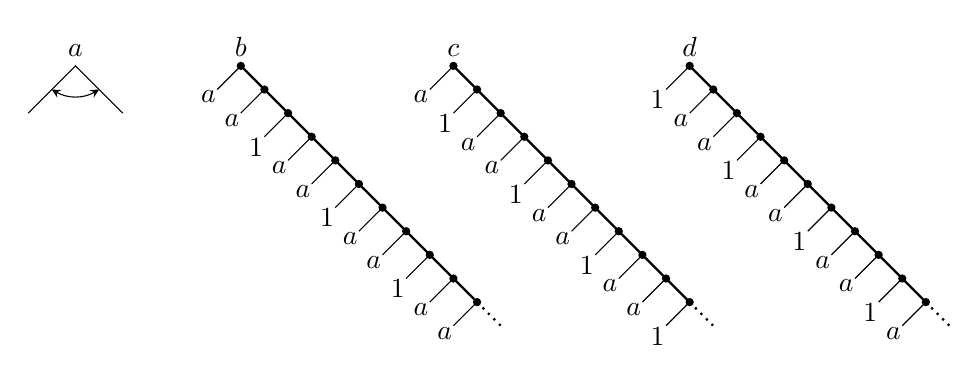
\begin{tikzpicture}[>=stealth,scale=0.3]
		
		\draw (0,0) -- (-2,2) node [above] {$a$} -- (-4,0);
		\draw [<->] (-3,1) to [bend right] (-1,1);
		
		\begin{scope}[shift={(7,0)}]
			\draw (0,0) -- (-2,2) node [above] {$b$} -- (8,-8);
			\foreach \x in {-2,-1,0,1,2,...,8} {
				\fill (\x,-\x) circle (5pt);
			}
			\foreach \x in {-2,-1,1,2,4,5,7,8} {
				\draw (\x,-\x) to +(-1,-1) node [below left=-0.3em] {$a$};
			}
			\foreach \x in {0,3,6} {
				\draw (\x,-\x) to +(-1,-1) node [below left=-0.3em] {$1$};
			}
			\draw [dotted,thick] (8,-8) to +(1,-1);
			\draw [thick] (-2,2) to (8,-8); 
		\end{scope}
		
		\begin{scope}[shift={(16,0)}]
			\draw (0,0) -- (-2,2) node [above] {$c$} -- (8,-8);
			\foreach \x in {-2,-1,0,1,2,...,8} {
				\fill (\x,-\x) circle (5pt);
			}
			\foreach \x in {-2,0,1,3,4,6,7} {
				\draw (\x,-\x) to +(-1,-1) node [below left=-0.3em] {$a$};
			}
			\foreach \x in {-1,2,5,8} {
				\draw (\x,-\x) to +(-1,-1) node [below left=-0.3em] {$1$};
			}
			\draw [dotted,thick] (8,-8) to +(1,-1);
			\draw [thick] (-2,2) to (8,-8); 
		\end{scope}
		
		\begin{scope}[shift={(26,0)}]
			\draw (0,0) -- (-2,2) node [above] {$d$} -- (8,-8);
			\foreach \x in {-2,-1,0,1,2,...,8} {
				\fill (\x,-\x) circle (5pt);
			}
			\foreach \x in {-1,0,2,3,5,6,8} {
				\draw (\x,-\x) to +(-1,-1) node [below left=-0.3em] {$a$};
			}
			\foreach \x in {-2,1,4,7} {
				\draw (\x,-\x) to +(-1,-1) node [below left=-0.3em] {$1$};
			}
			\draw [dotted,thick] (8,-8) to +(1,-1);
			\draw [thick] (-2,2) to (8,-8);
		\end{scope}
	\end{tikzpicture}
\end{document}